\section{Resultados}

\subsection{Desafíos de captura y fusión multicanal de imágenes térmicas}

Los videos capturados por las cámaras FLIR de la Fuerza Aérea Colombiana (FAC) enfrentaron una serie de desafíos técnicos derivados de las complejas condiciones de captura aérea en la región amazónica colombiana. Estas imágenes térmicas estuvieron afectadas por múltiples problemas de calidad que dificultaron su procesamiento automático. Entre los factores más críticos se identificaron: un elevado nivel de ruido térmico, generado por las fluctuaciones del sensor y las condiciones ambientales extremas; distorsiones producto del movimiento constante y las vibraciones de la aeronave; sombras pronunciadas que ocultaban parcialmente los objetos de interés; y una resolución limitada, afectada tanto por la densa atmósfera como por la distancia entre la cámara y el terreno.

Estas condiciones adversas se reflejaron directamente en los resultados obtenidos en una fase preliminar, donde los modelos de detección fueron aplicados sobre imágenes sin ningún tipo de preprocesamiento. En esta etapa inicial, el desempeño fue considerablemente deficiente, con dificultades notorias para detectar correctamente los elementos relevantes en las escenas. Estos resultados iniciales subrayaron la necesidad imperativa de implementar un conjunto de técnicas de preprocesamiento especializadas, destinadas a mejorar la calidad y la coherencia de las imágenes antes de su uso en algoritmos de detección de objetos. Dicha preparación previa se vuelve fundamental para maximizar la efectividad de los modelos y garantizar resultados fiables y robustos en este contexto tan desafiante.

En la Figura~\ref{Img:tratadas} se presenta una visualización del esquema de preprocesamiento diseñado, el cual se basa en la integración de información complementaria a través de una imagen RGB sintética. Cada uno de los tres canales fue generado mediante transformaciones dirigidas a resaltar aspectos específicos de la imagen, maximizando así la riqueza de la representación resultante.

\begin{itemize}
    \item El \textbf{canal rojo (R)} contiene la imagen suavizada tras aplicar una secuencia de filtros especializados: Gaussiano (para atenuar ruido global), Mediano (para eliminar ruido impulsivo sin afectar bordes), y Guiado (para conservar contornos estructurales relevantes). Esta combinación mejora significativamente la nitidez de las formas, permitiendo una mejor identificación de objetos lineales como carreteras o cuerpos de agua.
    
    \item El \textbf{canal verde (G)} representa una codificación textural obtenida a partir de un banco de filtros de Gabor. Estas funciones permiten capturar características orientadas, tales como rugosidad del terreno o variaciones de vegetación, útiles para segmentar regiones según su morfología superficial.
    
    \item El \textbf{canal azul (B)} incorpora una segmentación binarizada obtenida mediante el algoritmo Chan-Vese. Este procedimiento reduce la complejidad de la escena, facilita la eliminación de fondo y permite enfocar la atención del modelo en las regiones más relevantes.
\end{itemize}

La fusión de estos tres canales da lugar a una imagen RGB enriquecida que combina suavizado estructural, textura direccional y segmentación espacial. Esta representación multicanal resulta particularmente adecuada para ser utilizada como entrada en sistemas de detección de objetos, al ofrecer una visión más robusta, informativa y discriminativa de las escenas térmicas complejas propias del entorno amazónico.

\begin{figure}
\centering
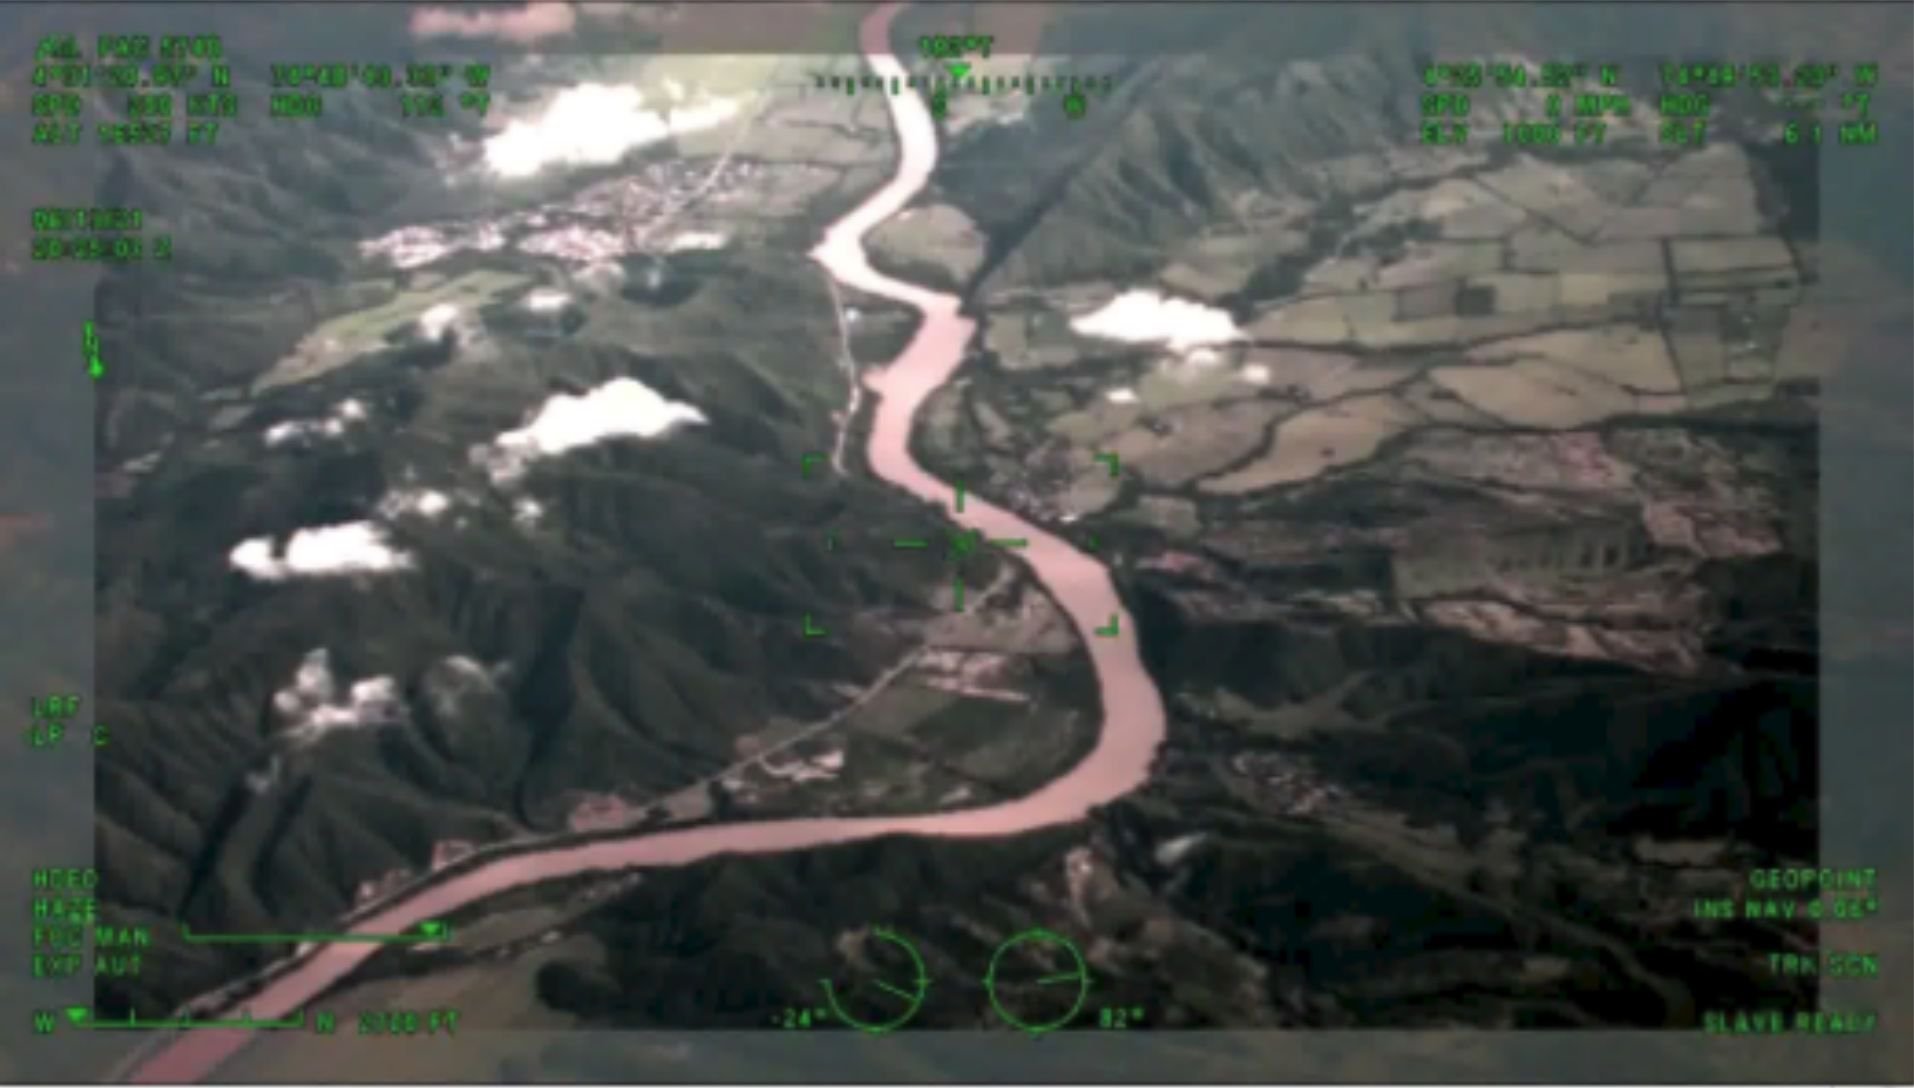
\includegraphics[width=0.6\linewidth]{figures/original.png}
\hfill
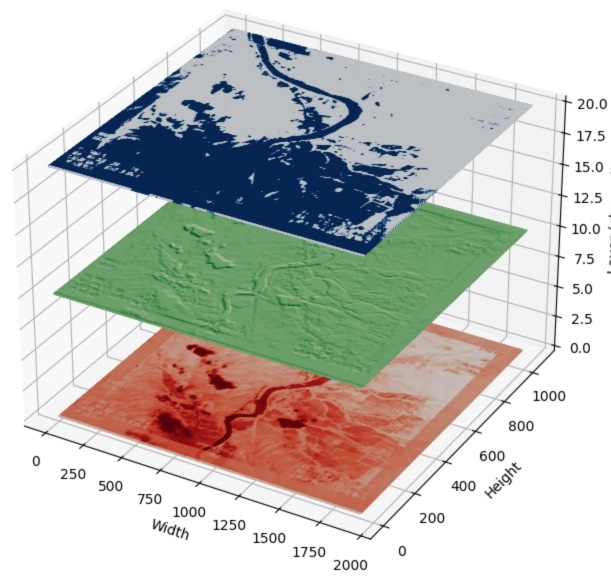
\includegraphics[width=0.7\linewidth]{figures/fusion.jpeg}
\hfill
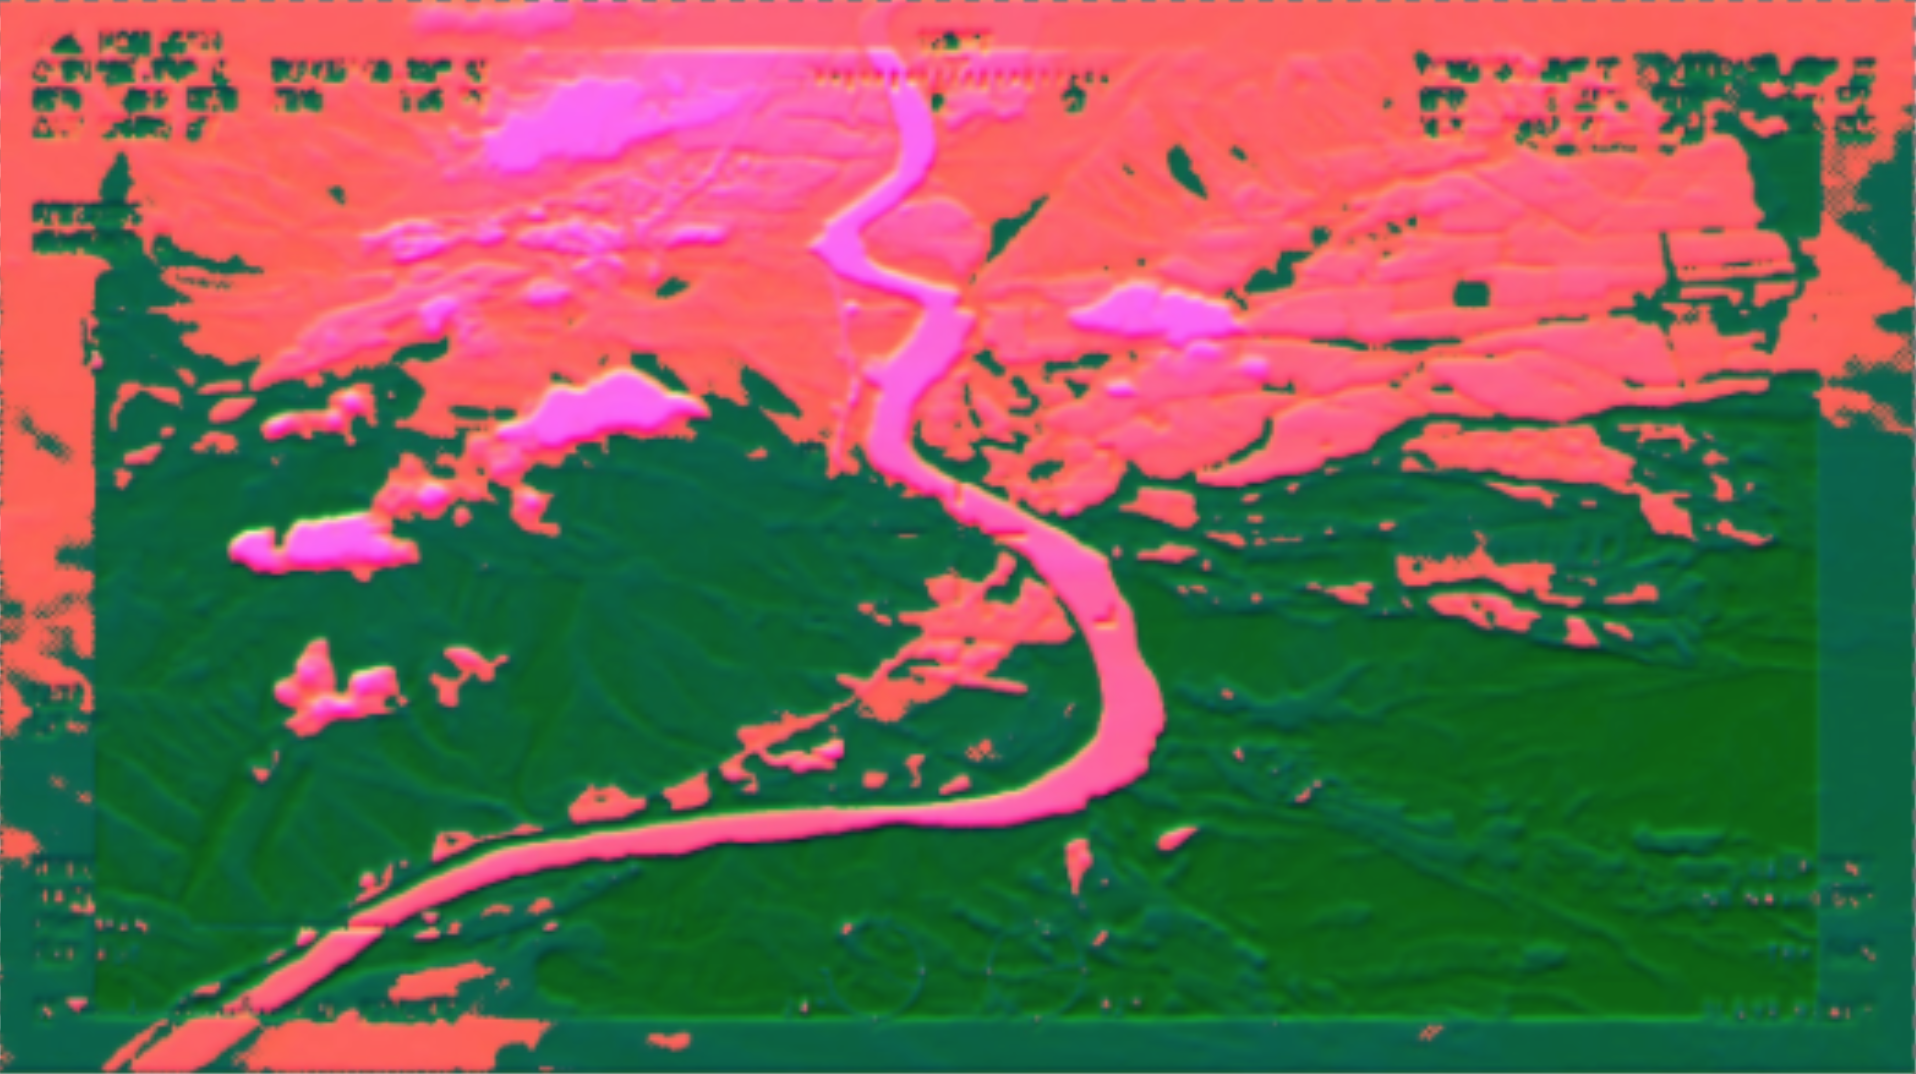
\includegraphics[width=0.6\linewidth]{figures/procesada.png}
\caption {Fusión multicanal de preprocesamiento. Arriba: Imagen original. Centro: canal azul (segmentación chan-vese binarizada), canal rojo (imagen suavizada sin ruido), canal verde (respuestas texturales de filtros de Gabor) Abajo: imagen RGB resultante de la combinación de canales.}

\label{Img:tratadas}
\end{figure}

\subsection{Impacto del Preprocesamiento en la Detección}

El esquema de preprocesamiento implementado demostró ser crucial para mejorar significativamente el rendimiento de los modelos de detección. Las transformaciones específicas aplicadas a cada canal (filtrado Gaussiano, Mediano y Guiado en el canal rojo; segmentación Chan-Vese en el canal azul; y codificación textural mediante filtros de Gabor en el canal verde) actuaron como un mecanismo de \textit{aumentación implícita} de los datos. Esta estrategia permitió enriquecer la representación de las imágenes sin necesidad de recurrir a técnicas tradicionales de \textit{data augmentation}.

Los resultados comparativos entre los modelos evaluados sobre imágenes originales (sin preprocesamiento) y preprocesadas muestran mejoras sustanciales en todos los casos, tanto en métricas estándar como en la capacidad de generalización de los modelos.

\vspace{1em}
\noindent\textbf{YOLO11s} (9.4 millones de parámetros):
\begin{itemize}
    \item \textbf{mAP@50:} de 33.7\% a 61.8\% (\textbf{+28.1 p.p.})
    \item \textbf{mAP@50-95:} de 12.6\% a 32.8\% (\textbf{+20.2 p.p.})
\end{itemize}

\noindent\textbf{YOLO11l} (25.3 millones de parámetros):
\begin{itemize}
    \item \textbf{mAP@50:} de 44.0\% a 65.2\% (\textbf{+21.2 p.p.})
    \item \textbf{mAP@50-95:} de 20.7\% a 32.1\% (\textbf{+11.4 p.p.})
\end{itemize}

\noindent\textbf{YOLO11l Fine-tuned} (ajustado con pesos específicos del dominio):
\begin{itemize}
    \item \textbf{mAP@50:} de 48.4\% a 51.7\% (\textbf{+3.3 p.p.})
    \item \textbf{mAP@50-95:} de 19.5\% a 24.9\% (\textbf{+5.4 p.p.})
\end{itemize}

\vspace{0.5em}
Estos resultados confirman que el preprocesamiento no solo mejoró la calidad visual de las imágenes térmicas, sino que también optimizó de manera efectiva el desempeño de los modelos de detección automática. La incorporación de información estructural, textural y segmentada en los canales RGB permitió una interpretación más robusta de las escenas, lo cual facilitó la detección precisa de elementos de interés como carreteras sin pavimentar y cuerpos de agua en entornos selváticos complejos.

\subsection{Evaluación Comparativa de Arquitecturas de Detección}

Tras los resultados positivos obtenidos con el esquema de preprocesamiento, se llevó a cabo una evaluación comparativa entre cinco arquitecturas modernas de detección de objetos. Para esta etapa, se emplearon exclusivamente imágenes preprocesadas, asegurando así condiciones óptimas de entrada para todos los modelos. Además de las variantes de YOLO11, se incluyeron dos arquitecturas ampliamente utilizadas en la literatura: Faster R-CNN y RetinaNet.

La Tabla~\ref{tab:resultados_modelos} resume los resultados obtenidos, ordenados en función del rendimiento alcanzado en la métrica \texttt{mAP@50}. Se reportan también los valores de \texttt{mAP@50-95} y el número de parámetros aproximado de cada modelo, lo cual proporciona una perspectiva adicional sobre su complejidad y eficiencia.

\begin{table}[h]
\centering
\small % Tamaño de fuente reducido
\caption{Rendimiento de arquitecturas evaluadas}
\label{tab:resultados_modelos}
\begin{tabular}{|l|c|c|c|}
\hline
\textbf{Modelo} & \textbf{Param. (M)} & \textbf{mAP@50} & \textbf{mAP@50--95} \\
\hline
YOLO11l & 25.3 & 65.2\% & 32.1\% \\
YOLO11s & 9.4 & 61.8\% & 32.8\% \\
Faster R-CNN & -- & 56.6\% & 32.8\% \\
YOLO11l FT & 25.3 & 51.7\% & 24.9\% \\
RetinaNet & 32.2 & 26.9\% & 12.2\% \\
\hline
\end{tabular}
\end{table}

Los resultados obtenidos muestran que las variantes del modelo YOLO11, tanto \texttt{YOLO11s} (versión \textit{small}) como \texttt{YOLO11l} (versión \textit{large}), se destacaron como las arquitecturas más eficaces en el contexto de imágenes térmicas procesadas. 

El modelo \texttt{YOLO11l}, con 25.3 millones de parámetros, alcanzó la mayor precisión en la métrica \texttt{mAP@50}, con un 65.2\%, lo que indica una alta tasa de detección correcta de objetos cuando se permite un margen de error de hasta un 50\% en la superposición entre la predicción y la anotación real (\textit{IoU}). Esta métrica, más permisiva, es útil para evaluar la capacidad general del modelo para localizar objetos, especialmente en escenarios donde el ruido o la resolución afectan la precisión de las cajas predichas.

No obstante, \texttt{YOLO11s}, con solo 9.4 millones de parámetros, mostró una eficiencia sobresaliente: obtuvo un \texttt{mAP@50--95} de 32.8\%, superando ligeramente a su contraparte más grande. Esta métrica promedia la precisión en múltiples umbrales de \textit{IoU} (desde 0.5 hasta 0.95, en incrementos de 0.05), y es más rigurosa, pues evalúa no solo la capacidad de detectar, sino también de localizar con precisión los objetos. El mejor resultado de \texttt{YOLO11s} en esta métrica sugiere una generalización más robusta y una mayor precisión espacial, a pesar de su menor complejidad computacional.

El modelo \texttt{Faster R-CNN} también presentó un rendimiento competitivo, con un \texttt{mAP@50--95} igual al de \texttt{YOLO11s} (32.8\%) y un \texttt{mAP@50} de 56.6\%. Aunque su precisión global fue inferior a la de los modelos YOLO11, su arquitectura de dos etapas demostró ser capaz de aprovechar el preprocesamiento aplicado, especialmente en términos de precisión detallada. En cambio, \texttt{RetinaNet}, con 32.2 millones de parámetros, obtuvo los valores más bajos tanto en \texttt{mAP@50} (26.9\%) como en \texttt{mAP@50--95} (12.2\%). Esto puede deberse a su mayor sensibilidad a condiciones adversas como el ruido térmico y el bajo contraste característicos de las imágenes FLIR.

\subsection{Desafíos Inherentes a las Imágenes FLIR}

A pesar de las mejoras sustanciales obtenidas mediante el preprocesamiento, los resultados alcanzados reflejan las limitaciones inherentes al trabajo con imágenes térmicas FLIR capturadas en condiciones operacionales reales. Este tipo de datos presenta desafíos particulares que afectan directamente el rendimiento de los algoritmos de detección:

\begin{itemize}
    \item \textbf{Variabilidad térmica:} Las diferencias de temperatura entre los objetos de interés y su entorno pueden ser mínimas, especialmente durante ciertos periodos del día, lo que dificulta la diferenciación clara de las clases.
    \item \textbf{Resolución limitada:} La distancia entre la aeronave y la superficie terrestre impone restricciones importantes sobre la resolución espacial, reduciendo la capacidad de distinguir detalles finos.
    \item \textbf{Condiciones atmosféricas adversas:} La humedad, nubosidad y partículas en suspensión características de la región amazónica degradan la señal térmica captada por los sensores, introduciendo ruido e inconsistencias.
    \item \textbf{Movimiento de plataforma:} Las vibraciones, oscilaciones y desplazamientos de la aeronave durante el vuelo generan distorsiones que afectan la estabilidad espacial de las imágenes, introduciendo artefactos que comprometen la detección.
\end{itemize}

Estos factores explican por qué, incluso tras aplicar un pipeline de preprocesamiento avanzado, los valores absolutos de \texttt{mAP} se mantienen por debajo de los estándares comúnmente reportados en tareas de detección sobre imágenes RGB convencionales. En consecuencia, se reafirma la necesidad de desarrollar enfoques personalizados y robustos, específicamente diseñados para operar eficazmente sobre imágenes térmicas aéreas en contextos naturales y de difícil acceso como la selva amazónica.


\subsection{Cumplimiento de Objetivos de Detección}

Los resultados obtenidos permiten afirmar que se cumplió satisfactoriamente el objetivo general del proyecto: desarrollar un modelo de detección automatizada basado en aprendizaje profundo para identificar carreteras y cuerpos de agua en imágenes térmicas FLIR capturadas por la Fuerza Aérea Colombiana. En particular, la arquitectura YOLO11l demostró ser la más efectiva, superando ampliamente las limitaciones de los enfoques tradicionales de análisis visual manual.

El modelo no solo logró detectar con precisión objetos de interés bajo condiciones operacionales reales, sino que también evidenció una mejora sustancial en su rendimiento gracias al esquema de preprocesamiento propuesto. En promedio, se observó un aumento de \textbf{17.5 puntos porcentuales en mAP@50}, lo que representa un avance significativo en la capacidad de interpretar escenas térmicas complejas.

Estos resultados confirman la viabilidad técnica de integrar soluciones de inteligencia artificial en los procesos de vigilancia aérea, y establecen una base robusta para futuras aplicaciones orientadas a la identificación temprana de actividades asociadas a minería ilegal u otras amenazas ambientales en la región amazónica. Asimismo, sientan las bases para la incorporación de este tipo de herramientas en sistemas operacionales de la FAC, mejorando la eficiencia y precisión en la toma de decisiones estratégicas.


\subsection{Despliegue}
El despliegue del sistema se realizó en dos partes: front-end y back-end.
La interfaz front-end, orientada al usuario final, fue desarrollada utilizando el framework Svelte, el cual se basa en JavaScript. Esta parte gestiona toda la interacción directa con el usuario, ofreciendo una experiencia ligera y responsiva. El código fuente del front-end está alojado en un repositorio público de GitHub y fue desplegado utilizando Vercel, una plataforma de hosting gratuita que se integra fácilmente con GitHub para facilitar el despliegue.

Por otro lado, el back-end se encarga de la lógica principal del sistema. Este servicio toma una imagen como entrada, determina el modelo de detección a aplicar y ejecuta el procesamiento correspondiente. Fue desarrollado en Python y hace uso de diversos frameworks y librerías para tareas de visión por computador, incluyendo PyTorch, Ultralytics (YOLO), entre otros.

El back-end no es de acceso público y se encuentra desplegado en un clúster de procesamiento de AWS (Amazon Web Services), utilizando una instancia tipo EC2 y recursos computacionales suficientes para el análisis de imágenes. La comunicación entre el front-end y el back-end se realiza a través de peticiones HTTP a una IP específica. Este enfoque modular permite escalar cada componente de manera independiente y garantiza un entorno seguro y eficiente para el procesamiento y la entrega de resultados. El diagrama que muestra la arquitectura de despliegue se muestra en la figura \ref{fig:despliegue}.


\begin{figure}
    \centering
    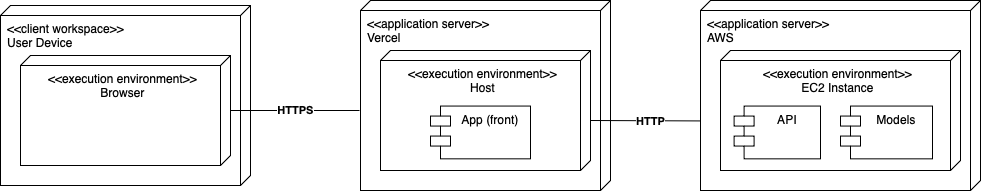
\includegraphics[width=1\linewidth]{figures/diagrama-despliegue.drawio.png}
    \caption{Diagrama de despliegue en UML}
    \label{fig:despliegue}
\end{figure}

Se puede apreciar un pantallazo del sistema en funcionamiento en la figura \ref{fig:pantallazo}, el despliegue se puede consultar a continuación en este enlace: \href{https://isis4825-proyecto-final.vercel.app}{https://isis4825-proyecto-final.vercel.app}


\begin{figure}
    \centering
    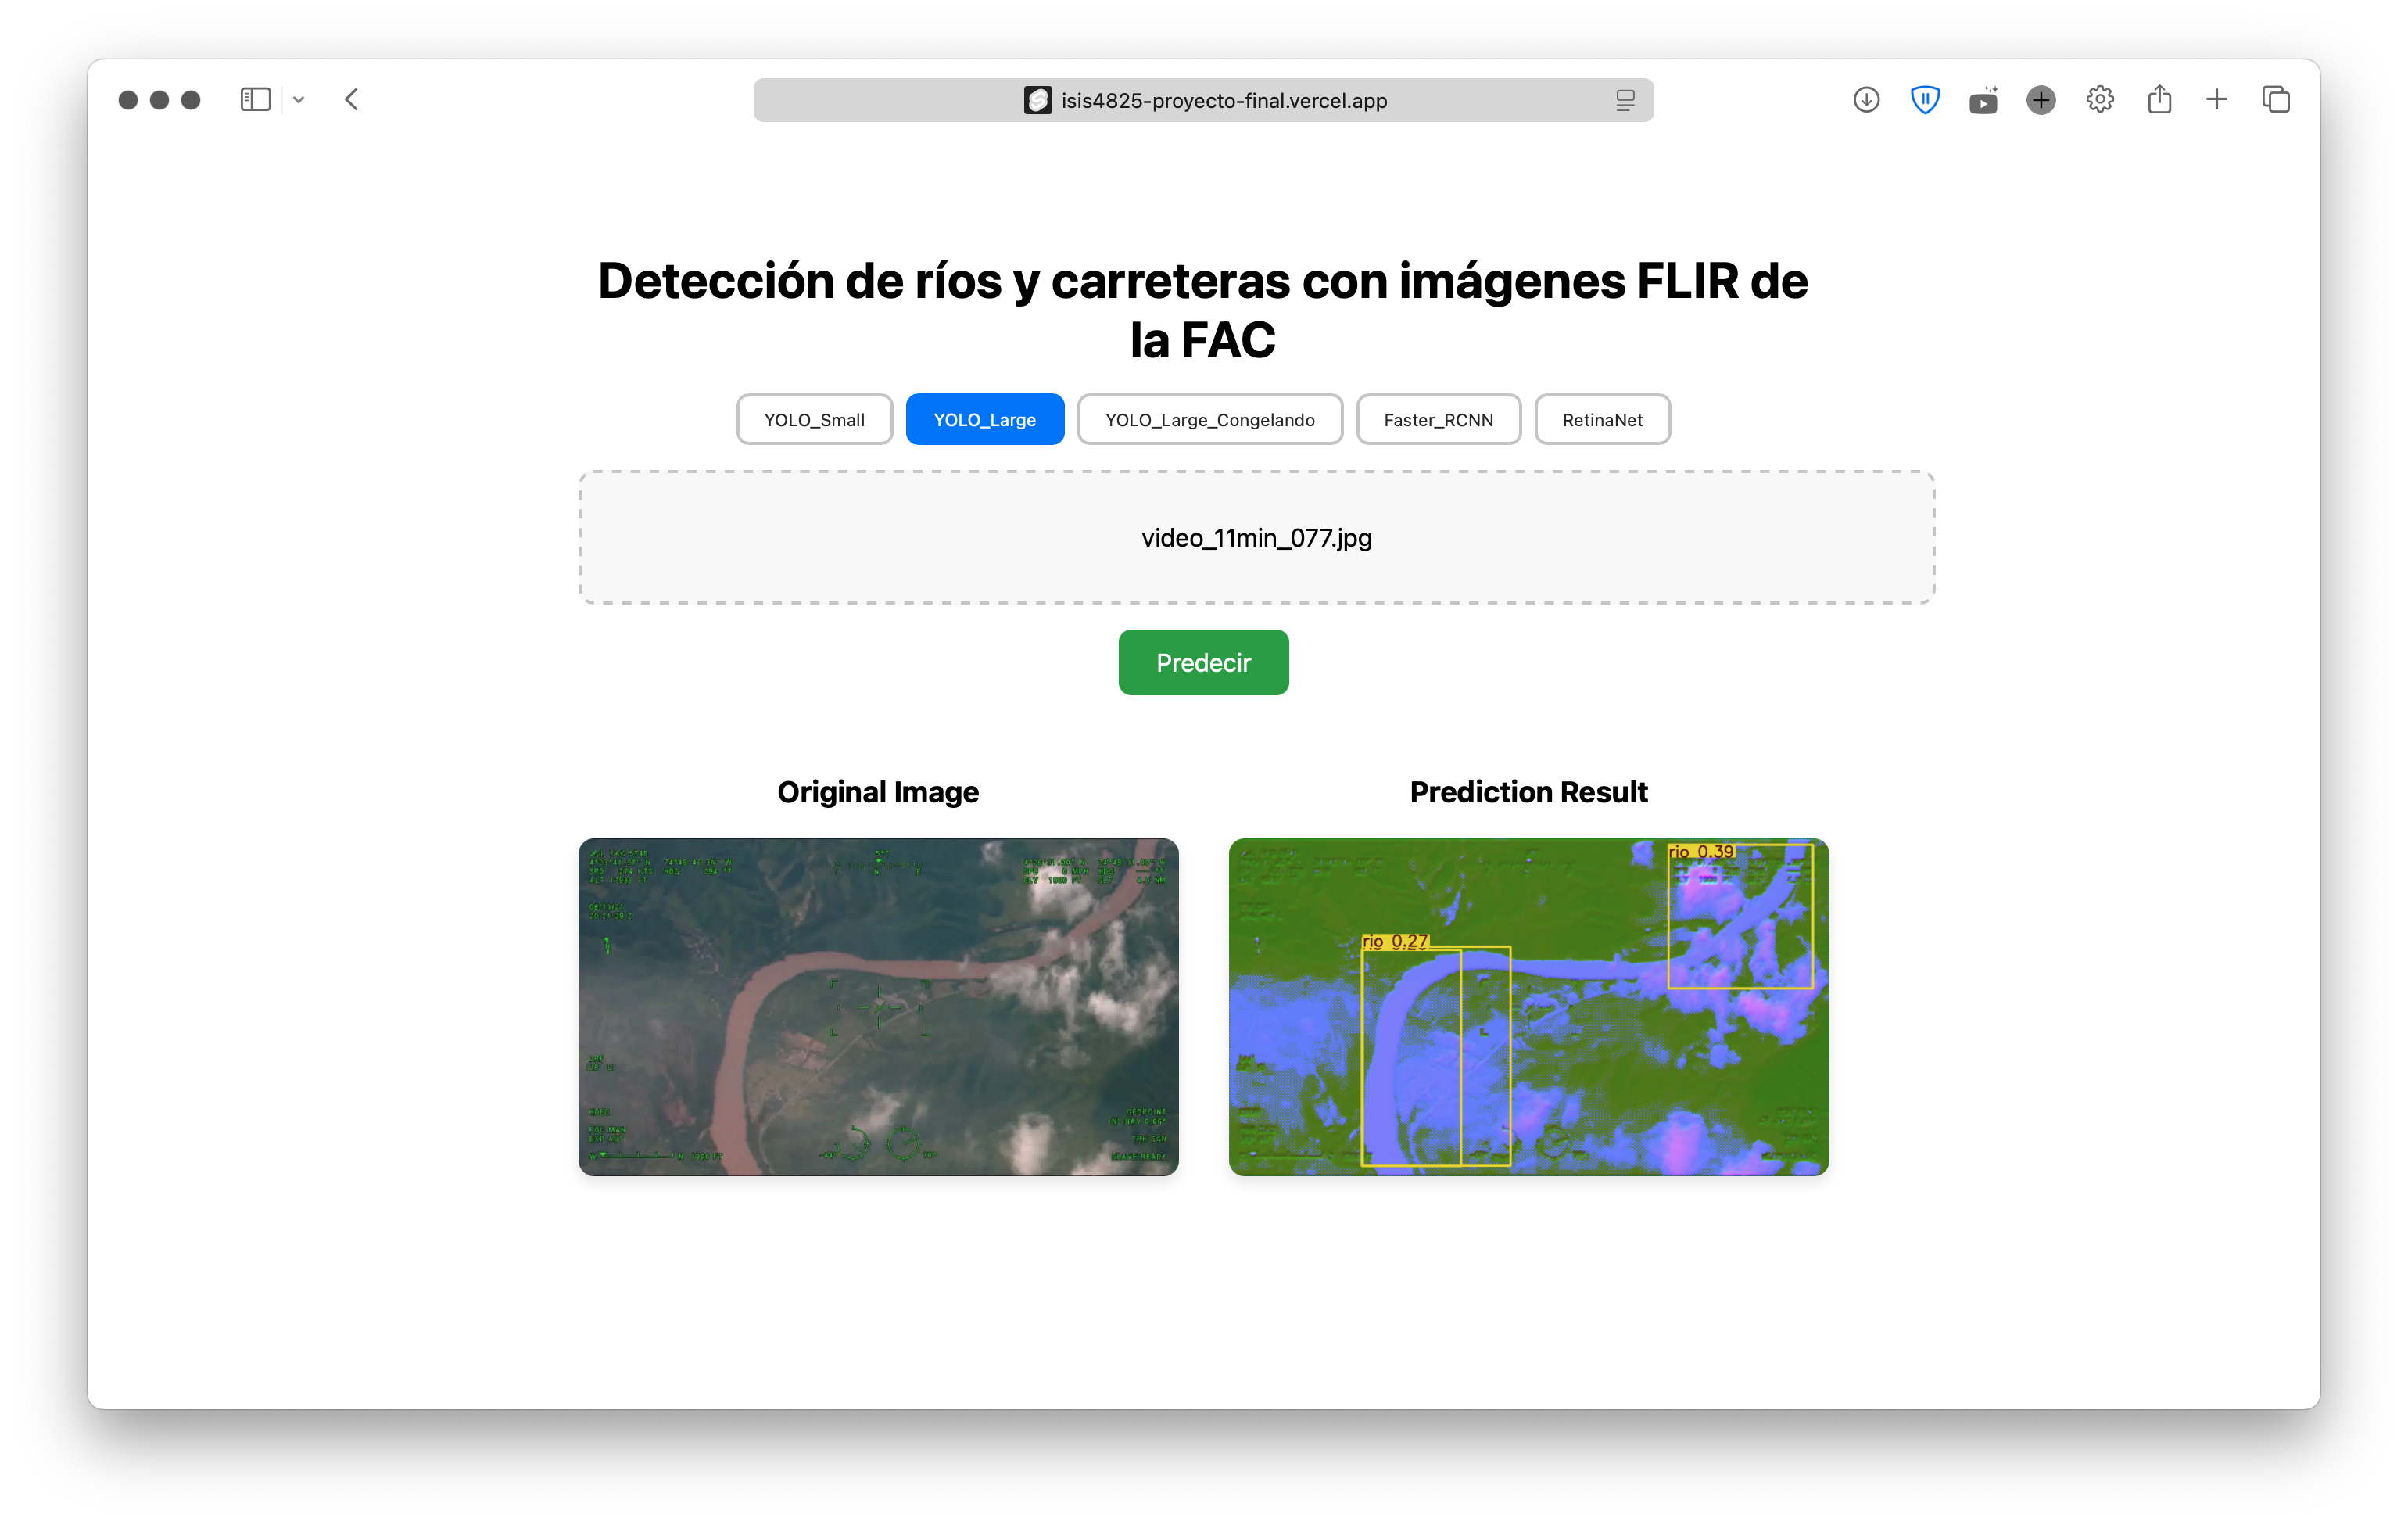
\includegraphics[width=1\linewidth]{figures/pantallazo.png}
    \caption{Pantallazo del despliegue en funcionamiento}
    \label{fig:pantallazo}
\end{figure}